% Copyright 2004 by Till Tantau <tantau@users.sourceforge.net>.
%
% In principle, this file can be redistributed and/or modified under
% the terms of the GNU Public License, version 2.
%
% However, this file is supposed to be a template to be modified
% for your own needs. For this reason, if you use this file as a
% template and not specifically distribute it as part of a another
% package/program, I grant the extra permission to freely copy and
% modify this file as you see fit and even to delete this copyright
% notice. 

\documentclass{beamer}
\usepackage{polski}
\usepackage[utf8]{inputenc}
\usepackage{eucal}

% There are many different themes available for Beamer. A comprehensive
% list with examples is given here:
% http://deic.uab.es/~iblanes/beamer_gallery/index_by_theme.html
% You can uncomment the themes below if you would like to use a different
% one:
%\usetheme{AnnArbor}
%\usetheme{Antibes}
%\usetheme{Bergen}
%\usetheme{Berkeley}
%\usetheme{Berlin}
%\usetheme{Boadilla}
%\usetheme{boxes}
%\usetheme{CambridgeUS}
%\usetheme{Copenhagen}
%\usetheme{Darmstadt}
%\usetheme{default}
%\usetheme{Frankfurt}
%\usetheme{Goettingen}
%\usetheme{Hannover}
%\usetheme{Ilmenau}
%\usetheme{JuanLesPins}
%\usetheme{Luebeck}
%\usetheme{Madrid}
%\usetheme{Malmoe}
%\usetheme{Marburg}
%\usetheme{Montpellier}
%\usetheme{PaloAlto}
%\usetheme{Pittsburgh}
%\usetheme{Rochester}
%\usetheme{Singapore}
%\usetheme{Szeged}
\usetheme{Warsaw}

\title{Logika intuicjonistyczna i izomorfizm Curry'ego Howarda}


\author{Julia Majkowska}
% - Give the names in the same order as the appear in the paper.
% - Use the \inst{?} command only if the authors have different
%   affiliation.


% - Use the \inst command only if there are several affiliations.
% - Keep it simple, no one is interested in your street address.

\date{21 Października 2018}
% - Either use conference name or its abbreviation.
% - Not really informative to the audience, more for people (including
%   yourself) who are reading the slides online

\subject{Theoretical Computer Science}
% This is only inserted into the PDF information catalog. Can be left
% out. 

% If you have a file called "university-logo-filename.xxx", where xxx
% is a graphic format that can be processed by latex or pdflatex,
% resp., then you can add a logo as follows:

% \pgfdeclareimage[height=0.5cm]{university-logo}{university-logo-filename}
% \logo{\pgfuseimage{university-logo}}

% Delete this, if you do not want the table of contents to pop up at
% the beginning of each subsection:
\AtBeginSubsection[]
{
  \begin{frame}<beamer>{}
    \tableofcontents[currentsection,currentsubsection]
  \end{frame}
}

% Let's get started
\begin{document}

\begin{frame}
  \titlepage
\end{frame}

\begin{frame}{}
  \tableofcontents
  % You might wish to add the option [pausesections]
\end{frame}

% Section and subsections will appear in the presentation overview
% and table of contents.
\section{Logika ituicjonistyczna}

\subsection{Wstęp}

\begin{frame}{Wstęp}
  \begin{itemize}
  \item {
   Logika oparta na konstukcji zmiennej
  }
  \item {
   Koncepcję przypisuje się matematykowi filozofowi Luitzen Egbertus Jan Brouwer (początek XX w)
  }
  \item {
   Formalna gałąź logiki od 1930r.
  }
  \end{itemize}
\end{frame}

\begin{frame}{Semantyka}
 \begin{block}{Interpretacja BHK zasad tworzenia formuł}
 \begin{enumerate}
  \item  Konstrukcja \(\phi_1 \wedge \phi_2  \) składa się z konstrukcji \(\phi_1\) i \(\phi_2\).
  \item  Konstrukcja \(\phi_1 \vee \phi_2  \) składa się z kostukcji \( i \in \{ 1, 2 \}\) i  \(\phi_i\).
  \item  Konstrukcja \(\phi_1 \rightarrow \phi_2  \) to funkcja zamieniająca konstrukcje \(\phi_1\) na konstrukcje \(\phi_2\).
  \item \( \bot\) oznacza brak konstrukcji.
  \item \( \neg \phi \) to skrócony zapis \( \phi \rightarrow \bot\)
 \end{enumerate}
   
\end{block}

\begin{example}
	\begin{enumerate}
	\item \(\bot \rightarrow \phi\)
	\item \( p \rightarrow \neg \neg p\)
	\end{enumerate}
\end{example}
\end{frame}

\begin{frame}{Semantyka}
 \begin{block}{Konwencje zapisu formuł}
 \begin{enumerate}
  \item  \( \neg p \) to skrót dla \( p \rightarrow \bot\)
  \item \( p\leftrightarrow q \) to skrót dla \( (p \rightarrow q ) \wedge ( q \rightarrow p ) \)
  \item  \( \rightarrow \) wiąże do prawej i ma najniższy priorytet
  \item  \( \neg \) ma najwyższy proprytet
  \item \( \wedge \) i \( \vee \) wiążą do lewej i mają ten sam priorytet
  \item Nie piszemy najbardziej zewnętrznych nawiasów
 \end{enumerate}
\end{block}

\begin{example}
\(\neg p \wedge q  \rightarrow r \Leftrightarrow (((\neg p ) \wedge q )  \rightarrow r) \)
\end{example}
\end{frame}

\subsection{Dedukcja Naturalna}
\begin{frame}{Dedukcja naturalna logiki intuicjonistycznej}
 \begin{block}{Oznaczenia}
 \begin{enumerate}
  \item PV - zbiór wszystkich zmiennych
  \item \( \Phi ::= \bot | PV | ( \Phi \rightarrow \Phi ) | ( \Phi \vee \Phi ) | ( \Phi \wedge \Phi ) \) - zbiór formuł
  \item  Kontekst to skończony podzbiór \( \Phi \).Będziemy używali \(\Gamma\) i \(\Delta \) do oznaczania kontekstów
  \item  \( \Gamma \vdash p \) intuicyjnie oznacza, że p wynika z założeń \( \Gamma\).
  \item Zamiast \( \Gamma \cup \Delta \) będziemy pisać \(\Gamma\), \(\Delta\), a zamiast \( \{\} \vdash p \) będziemy pisać \( \vdash p \).
  \item Formalnym dowodem \( \Gamma \vdash p \) jest drzewo,  w którym \( \Gamma \vdash p \) jest korzeniem, liśćmi są axiomy, a przejścia od ojca do syna odbywają się zgodnie z niżej podanymi zasadmi.
  \item Jeśli \( \vdash p \) to p jest tautologią logiki inuicjonistycznej
 \end{enumerate}
 \end{block}
 \end{frame}
 
\begin{frame}{Dedukcja naturalna logiki intuicjonistycznej}
 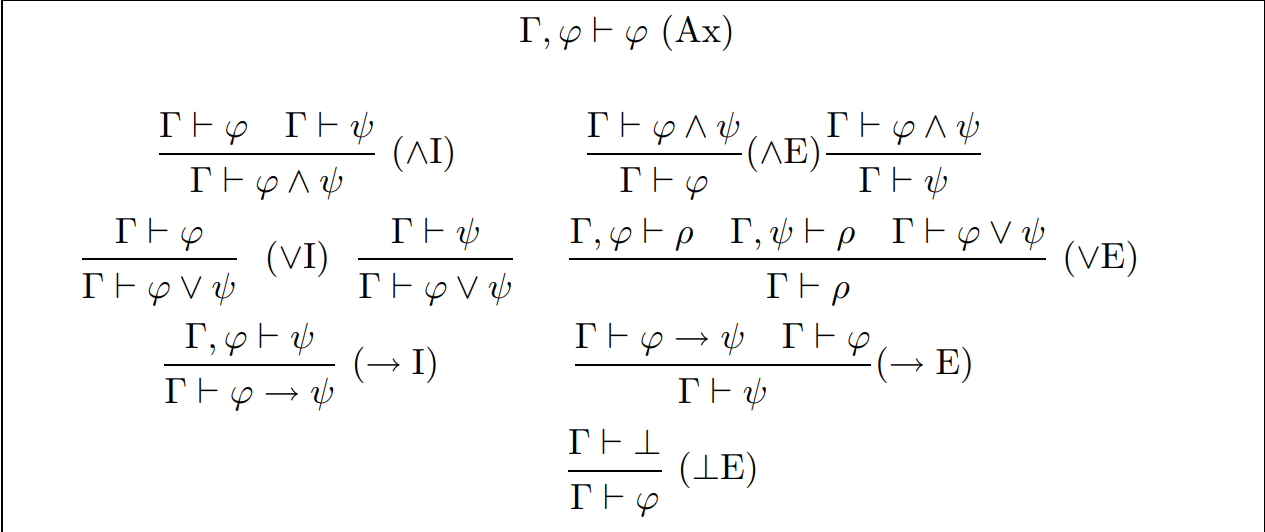
\includegraphics[scale=0.25]{dedukcja.png}
\end{frame}

\begin{frame}{Przykłady dowodów}
 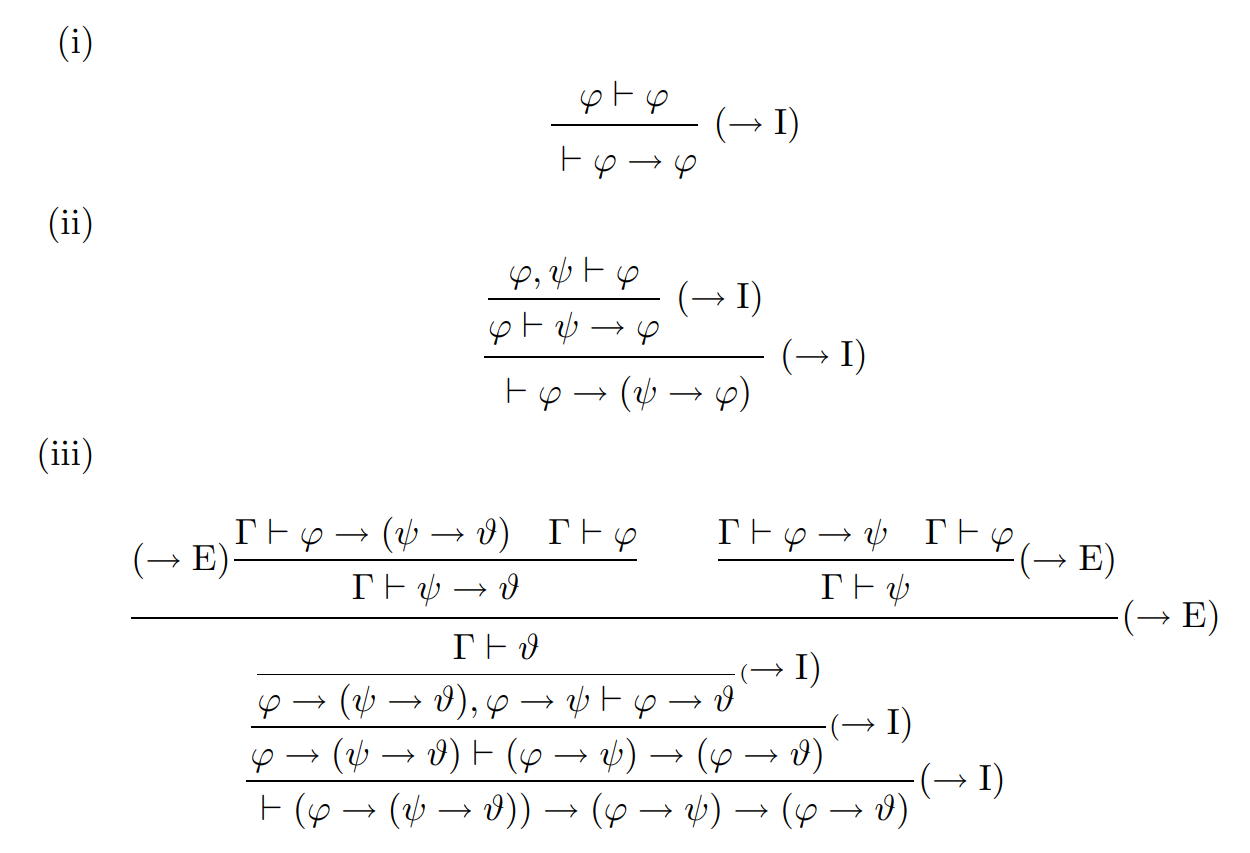
\includegraphics[scale=0.25]{dowoddedukcja.png}
\end{frame}

\begin{frame}{Własności dedukcji}
 \begin{block}{Lemat}
 	Logika intuicjonistyczna jest zamknięta na osłabienie i podstawienie. To znaczy : \\
 	\( \Gamma \vdash p \Rightarrow \Gamma, \psi \vdash p\)\\
 	\( \Gamma \vdash p  \Rightarrow \Gamma [ q := \psi ] \vdash p[ q:= \psi ]\)\\
 	Dowód - indukcja
 \end{block}
\end{frame}

\subsection{Algebraiczna Semantyka}

\begin{frame}{Logika klasyczna}
 \begin{block}{Wartościowanie dla logiki klasycznej}
 Niech \( v : \Phi \rightarrow \{0,1\}\)\\
 Zdefinujemy funkcję mapującą  \( [ \cdot ]_v : \Phi \rightarrow \{ 0, 1 \}\), spełniającą :
 \begin{equation*}
 	[p]_v = v ( p)
 \end{equation*} 
 \begin{equation*}
 	[\bot]_v = 0
 \end{equation*} 
  \begin{equation*}
 	[\phi \vee \psi]_v = max\{[\phi]_v, [\psi]_v\}
 \end{equation*}
  \begin{equation*}
 	[\phi \wedge \psi]_v = min\{[\phi]_v, [\psi]_v\}
 \end{equation*}
  \begin{equation*}
 	[\phi \rightarrow \psi]_v = max\{1-[\phi]_v, [\psi]_v\}
 \end{equation*}
 	
 \end{block}
\end{frame}


\begin{frame}{Ciało zbiorów}
 \begin{block}{Definicja}
 \textbf{Ciało zbiorów} nad X to niepusta rodzina pozdbiorów X zamknięta na sumę, przecięcie i dopełnienie zbiorów
 \end{block}
 \begin{example}
 \begin{enumerate}
 \item P(X)
 \item \( \{\{\}\} \cup X\)
 \end{enumerate}
 \end{example}
\end{frame}

\begin{frame}{Algebra zbiorów}
 \begin{block}{Wartościowanie na zbiorach}
 
 Niech \( \mathcal{R} \) ciało zbiorów nad zbiorem X.\\  	Wartosciowaniem v w \( \mathcal{R} \) nazywamy \( v : PV \rightarrow \mathcal{R}\)\\
 Zdefinujemy funkcję mapującą  \( [ \cdot ]_v : \Phi \rightarrow X\), spełniającą :
 \begin{equation*}
 	[p]_v = v ( p)
 \end{equation*} 
 \begin{equation*}
 	[\bot]_v = \{\}
 \end{equation*} 
  \begin{equation*}
 	[\phi \vee \psi]_v = [\phi]_v \cup [\psi]_v
 \end{equation*}
  \begin{equation*}
 	[\phi \wedge \psi]_v = [\phi]_v \cap [\psi]_v 
 \end{equation*}
  \begin{equation*}
 	[\phi \rightarrow \psi]_v = X-[\phi]_v \cup [\psi]_v
 \end{equation*}
 	
 \end{block}
 
\end{frame}

\begin{frame}

\begin{block}{Twierdzenie}
 	Powyższe dwie semantyki są równoważne.\\ \( \phi\) jest tautologią \( \Leftrightarrow \) \(v(\phi) = X \) dla każdego v w \(\mathcal{R}\).
 \end{block}
 \begin{block}{Dowód}
 
	\( \Rightarrow \)\\
	Załóżmy nie wprost, że istnieje a takie, że \( a \notin v(\phi)\). Więc tworzymy wartościowanie zmiennych w PV takie, że w(p) = 1 wtw. gdy \( a \in v(p)\). Indukcyjnie można udowodnić że \(w(\phi) \neq 1\).\\
	\( \Leftarrow \) \\
	Wartościowanie 0/1 kowe to interpretacja \( v (\phi) \in \{\{\}, X\} \).
 \end{block}
 
\end{frame}

\begin{frame}{Algebra boolowska}
 \begin{block}{Definicja}
 \textbf{Algebrą boolowską} nazywamy \( \mathcal{B}  = < B, \cup, \cap, -, 0, 1 >\), gdzie: 
 \begin{enumerate}
 \item \(\cup, \cap\) są łączne, przemienne i rozdzielne jedno względem drugiego.
 \item \( a \cup 0 = a \) i \( a \cap 1 = a \) 
 \item \( -a \cup a = 1 \) i \( -a \cap a  =  0 \)
 \end{enumerate}
 Relacja \(a \leq b  \Leftrightarrow  a \cup b = b \) jest częściowym porządkiem dla wszyskich algebr boolowskich. \( \cup \) \( \cap \) są odpowiednio infimum (glb) i supremum (lub) na tym porządku.
 \end{block}
 
\end{frame}

\begin{frame}{Algebra Lindenbauma}
 \begin{block}{Definicja}
 Niech \( \Phi \) - zbiór wszystkich formuł i \( \Gamma \in \Phi \) 
 
 Zdefiniujmy relację  \( \phi \sim \psi \Leftrightarrow (\Gamma, \phi  \vdash \psi) \wedge (\Gamma, \psi \vdash \phi) \).
 Relacja jest relacją równoważności ponieważ następujące formuły są dowodliwe: 
 \begin{enumerate}
 \item \(\phi \rightarrow \phi\)
 \item \((\phi \rightarrow \psi) \rightarrow (( \psi \rightarrow  \gamma ) \rightarrow ( \phi \rightarrow \gamma ))  \) 
 \end{enumerate}
 \end{block}
 
 \begin{block}{Zbiór Lindenbauma}
 
 Niech \( \mathcal{L}_{\Gamma} = \Phi / \sim  = \{ [\phi]_{\sim} :  \phi \in \Phi \}\). \\
 Zdefiniujmy częściowy porządek \( [\phi]_{\sim} \leq [\psi]_{\sim} \Leftrightarrow \Gamma, \phi \vdash \psi \)

 \end{block}
 
\end{frame}

\begin{frame}{Algebra Lindenbauma }
 \begin{block}{Operatory}
 Możemy zdefiniować dodatkowe operatory nad \( \mathcal{L}_{\Gamma} \)
 \begin{enumerate}
 \item \([\alpha]_{\sim} \cup [\beta]_{\sim} = [ \alpha \vee \beta ]_{\sim}\)
 \item \([\alpha]_{\sim} \cap [\beta]_{\sim} = [ \alpha \wedge \beta ]_{\sim}\)
  \item \(-[\alpha]_{\sim} = [\neg \alpha ]_{\sim}\)
  \item \( 1 = [\bot \rightarrow \phi ]_{\sim} \) , \( 0 = [\bot]_{\sim} \)
 \end{enumerate}
 \end{block}
 
  \begin{block}{Dowód}
 Operatory są dobrze zdefiniowane ponieważ następujące fomuły są dowodliwe
 \begin{enumerate}
 \item \((\alpha \rightarrow \alpha') \rightarrow 
 (
 	(\beta \rightarrow \beta') \rightarrow
 	(( \alpha \vee \beta) \rightarrow (\alpha' \vee \beta')))\)
  \item \((\alpha \rightarrow \alpha') \rightarrow 
 (
 	(\beta \rightarrow \beta') \rightarrow
 	(( \alpha \wedge \beta) \rightarrow (\alpha' \wedge \beta')))\)
  \item \((\alpha \rightarrow \alpha') \rightarrow 
(\neg \alpha' \rightarrow \neg \alpha)\)
 \end{enumerate}
 \end{block}
 
\end{frame}

\begin{frame}{Algebra Lindenbauma }
 \begin{block}{Twierdzenie}
 \( \cup \) i \(\cap \) są łączne, przemienne i rozdzielne oraz są operatorami lub i glb na porządku \( \leq \).
 \end{block}
 
\end{frame}

\begin{frame}{Algebra Heytinga}
 \begin{block}{Definicja}
\textbf{Algebrą Heytinga} nazywamy system algebraiczny w postaci \( \mathcal{H} = < H, \cup, \cap, \Rightarrow, - , 0 ,1 > \) spełniający 
\begin{enumerate}
	\item \(\cup, \cap\) są łączne, przemienne i rozdzielne jedno względem drugiego.
 \item \( a \cup 0 = a \) i \( a \cap 1 = a \) 
 \item \( a \cup a  = a \) 
 \item \( a \cap c \leq b \) jest równoważne \( c \leq a \Rightarrow b \) ( gdzie \( a \leq b \) to \( a \cup b  = b\) )
 \item \( -a  = a \Rightarrow 0 \)
\end{enumerate}
 \end{block}
\end{frame}
 
\begin{frame}{Algebra Heytinga}
 \begin{block}{Definicja}
 Niech \( \mathcal{H} = < H, \cup, \cap, \Rightarrow, - , 0 ,1 >  \) będzie algebrą Heytinga.\\
  Wartosciowaniem v w \( \mathcal{H} \) nazywamy \( v : PV \rightarrow H\)\\
 Zdefinujmy funkcję mapującą  \( [ \cdot ]_v : \Phi \rightarrow H\), spełniającą :
 \begin{equation*}
 	[p]_v = v ( p)
 \end{equation*} 
 \begin{equation*}
 	[\bot]_v = 0
 \end{equation*} 
  \begin{equation*}
 	[\phi \vee \psi]_v = [\phi]_v \cup [\psi]_v
 \end{equation*}
  \begin{equation*}
 	[\phi \wedge \psi]_v = [\phi]_v \cap [\psi]_v 
 \end{equation*}
  \begin{equation*}
 	[\phi \rightarrow \psi]_v = [\phi]_v \Rightarrow [\psi]_v
 \end{equation*}
 \end{block}
\end{frame}

\begin{frame}{Dowodliwość a algebra Heytinga}
 \begin{block}{Twierdzenie}
Następujące zdania sa równoważne
	\begin{enumerate}
	\item \(\Gamma \vdash \phi\)
 	\item \(\Gamma \models \phi\) tzn. \( \forall_{\mathcal{C}, v} ( \forall_{\gamma \in \Gamma} v(\gamma) = 1 ) \Rightarrow v(\phi)  = 1\)

	\end{enumerate}
 \end{block}
 
 \begin{block}{Twierdzenie}
	\begin{enumerate}
	\item Formuła \(\phi\) o długości n jest dowodliwa jeśli jest prawdziwa we wszystkich algebrach Heytinga o liczności nie większej niż \( 2 ^ {2 ^ n}\)
 	\item Niech \(\mathcal{H}\) będzie algebrą wszystkich podzbiorów gestej przestrzeni metrycznej. \( \mathcal{H} \models \phi\) wtw. gdy \(\phi\) jest prawdziwe.

	\end{enumerate}
 \end{block}
\end{frame}

\begin{frame}{Model Kripkego}
 \begin{block}{Definicja}
Jeśli \( \mathcal{C} = < C, \leq, \Vdash, f >\) jest \textbf{modelem Kripkego} wtedy : 
\begin{enumerate}
	\item \( f : PV \rightarrow C\)  \( f(p) = inf\{c \in C : c \Vdash p\}\) - wartościowanie ziennych
	\item \(c \Vdash \phi \vee \psi \Leftrightarrow c \Vdash  \phi \) lub \( c \Vdash \psi \) 
 \item \(c \Vdash \phi \wedge \psi \Leftrightarrow c \Vdash  \phi \) i \( c \Vdash \psi \) 
 \item \(c \Vdash \phi \rightarrow \psi \Leftrightarrow c' \Vdash  \psi \) dla każdego c', takiego że \( c \leq c'  c' \Vdash \phi \) 
 \item \( c \Vdash \bot \) nie jest prawdą
 
\end{enumerate}
 \end{block}
 
  \begin{block}{Wnioski}

\begin{enumerate}

 \item \(c \Vdash \neg \phi \Leftrightarrow  c'\nVdash \phi\) dla każdego \( c' \geq c\).

 \item \(c \leq c' \wedge  c \Vdash \phi \Rightarrow c' \Vdash \phi \)
\end{enumerate}
 \end{block}
\end{frame}


\begin{frame}{Zupełność}
 \begin{block}{Twierdzenie}
Poniższe zdanie są równoważne
\begin{enumerate}
\item \( \Gamma \vdash \phi \)
\item \( c \Vdash \Gamma \Rightarrow c \Vdash \phi \)
\end{enumerate}
 \end{block}
 
\end{frame}

\subsection{Fragment implikacyjny}

\begin{frame}{Logika inuicjonistyczna z samą impllikacją}
 \begin{block}{Twierdzenie}
Rachunek zdań z samą implikacją jest zupełny w kontekscie modelu Kripkego. : 
\begin{enumerate}
\item \( \Gamma \vdash \phi \)
\item \( \mathcal{C} \Vdash \Gamma \Rightarrow \mathcal{C} \Vdash \phi \)
\end{enumerate}
są równoważne.
	
 \end{block}
 
  \begin{block}{Twierdzenie}
  Niech \(\phi\) zdanie implikacyjne, a \(\Gamma\) zbiór formuł implikacyjnych. Jeśli \( \Gamma \vdash \phi \) jest prawdą w rachunku intuicjonistycznym to jest też prawdą w rachunku z samymi implikacjami. 

 \end{block}
\end{frame}

\section{Izomorfizm Curry'ego Howarda}

\subsection{Bezkontekstowa dedukcja naturalna}
\begin{frame}{Dedukcja bez kontekstu}
Założenia są umieszczane w liściu drzewa i uwalniane w momencie kiedy stosujemy w dowodzie wprowadzenie implikacji.
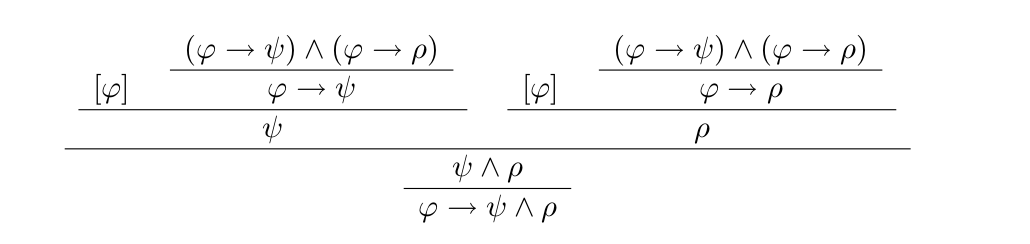
\includegraphics[scale=0.25]{bezkontdedukcja.png}
\end{frame}

\begin{frame}{Normalizacja dowodów}
Niektóre dowody wprowadzają nowe spójniki, tylko po to, żeby je wyeliminować później
\begin{example}
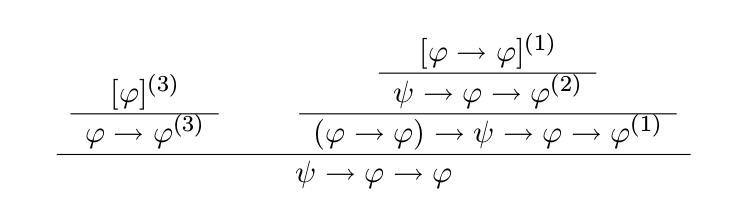
\includegraphics[scale=0.25]{duzy_dowod.png}
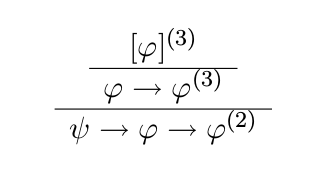
\includegraphics[scale=0.25]{maly_dowod.png}
\end{example}
\end{frame}

\begin{frame}{Normalizacja dowodów}

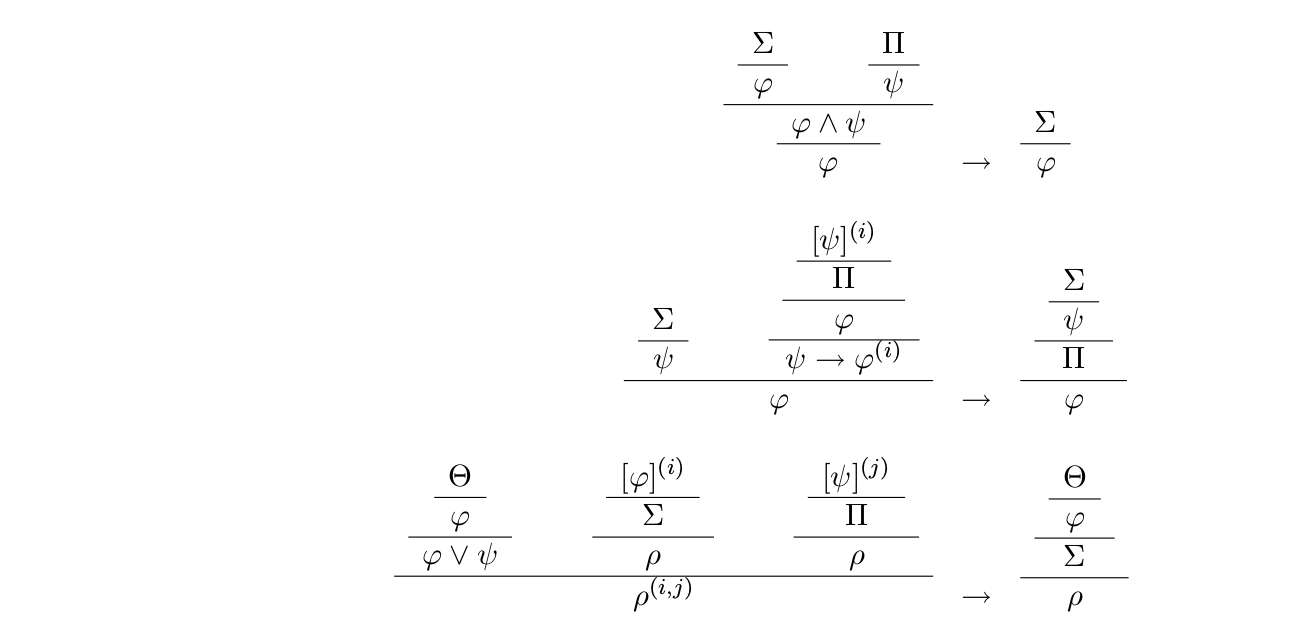
\includegraphics[scale=0.25]{elim_ded.png}

\end{frame}

\subsection{Izomorfizm Curry'ego Howarda}
\begin{frame}{Izomorfizm Currego Howarda}
\begin{block}{Twierdzenie}

Będziemy rozpatrywać część implikacyjną logiki inuicjonistycznej. 
\begin{enumerate}
	\item Jeśli \( \Gamma \vdash M : \phi \) to \( | \Gamma | \vdash \phi \) gdzie \(|\cdot|\) oznacza zbiór typów zbioru zmiennych.
	\item Jeśli \( \Gamma \vdash \phi \) to istnieje \( M \in \Lambda_{\pi}\) takie, że \( \Delta \vdash M : \phi \) gdzie \( \Delta = \{ (X_{\phi} : \phi) | \phi \in \Gamma \} \)
\end{enumerate}
Dowód - indukcja po konstrukcji formuły / dowodu.
\end{block}
\end{frame}

\begin{frame}{Izomorfizm Currego Howarda a logika intuicjonistyczna}
Aby rozszerzyć izomorfizm do pełnego rachunku zdań logiki intuicjonistycznej należy dołożyć następujące typy do prostego typowango rachunku lambda.
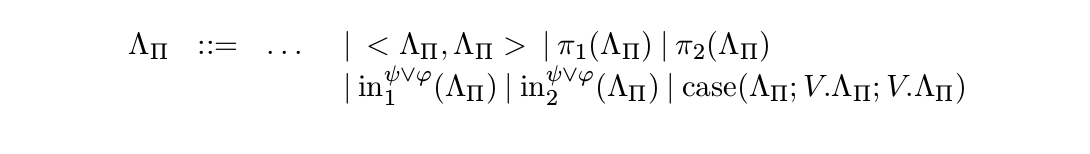
\includegraphics[scale=0.25]{types_curry.png}
\end{frame}

\begin{frame}{Izomorfizm Currego Howarda a logika intuicjonistyczna}
Należy dołożyć także dodatkowe zasady typowanie i redukcji
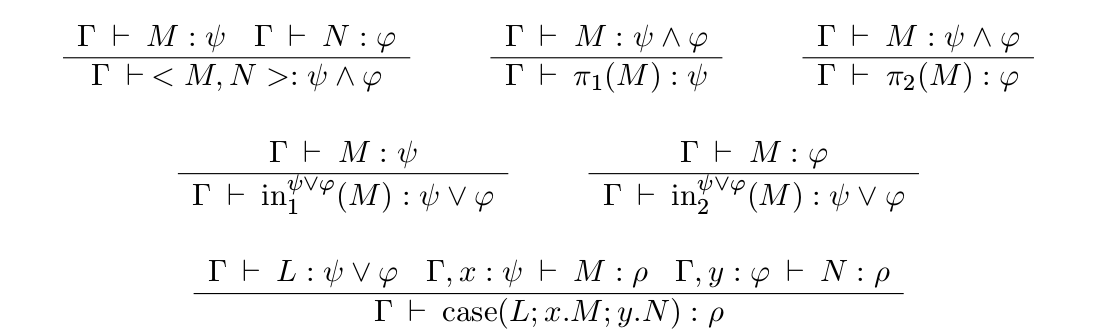
\includegraphics[scale=0.25]{int_curry.png}\\
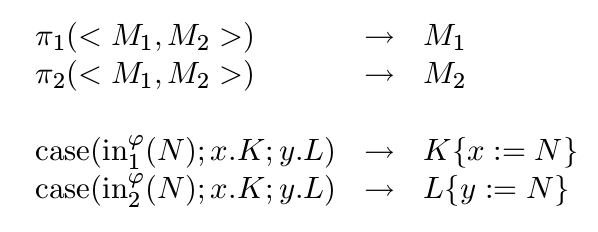
\includegraphics[scale=0.25]{red_curry.png}
\end{frame}

\begin{frame}{Przedstawienie dowodu jako \(\lambda\) termu}
Można zauważyć podobieństwa pomiędzy cechami dowodu a cechami \(\lambda\) -termu.

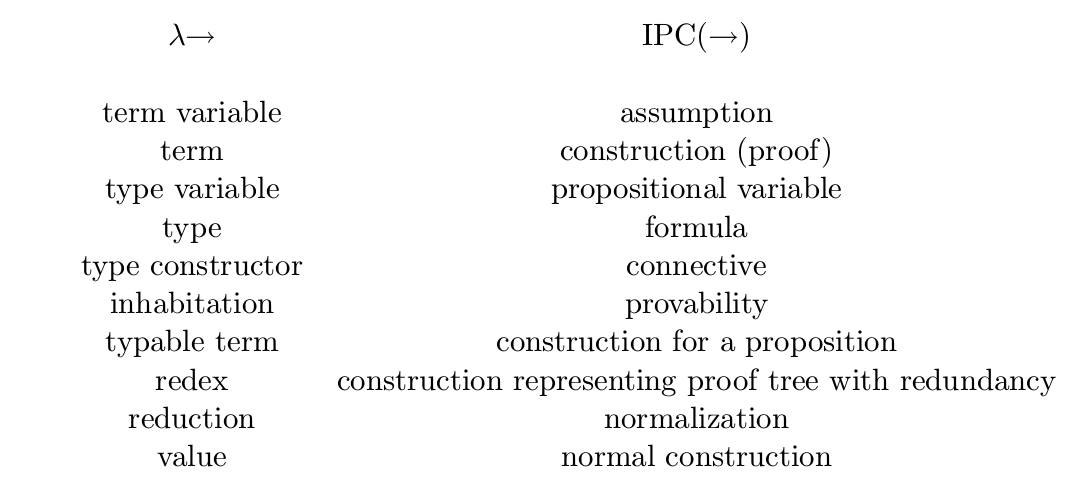
\includegraphics[scale=0.25]{odpowiedniki_curry.png}
\end{frame}

\begin{frame}{Przedstawienie dowodu jako \(\lambda\) termu - redukcja}
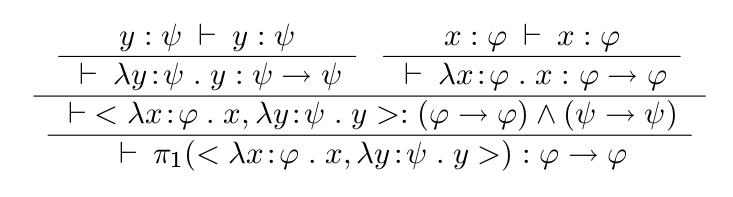
\includegraphics[scale=0.25]{redex_curry.png}
\end{frame}

\begin{frame}{Własność silnej redukcji}
\begin{block}{Twierdzenie}
	Każda redukcja  termu typowanego rachunku lambda ma skończoną długość.

\end{block}
\end{frame}

\subsection{Ćwiczenia}

\begin{frame}{Ćwiczenia}
\begin{enumerate}

	\item Udowodnij w systemie dedukcji naturalnej używając termów logiki inuicjonistycznej. Staraj się aby powstały dowód był znormalizowany.
	\begin{enumerate}
 \item \( \bot \rightarrow p\)
 \item \( p \rightarrow \neg \neg p \)
 \item \( \neg \neg \neg p \rightarrow \neg p\)
 \item \( (p \rightarrow q) \rightarrow (\neg q \rightarrow \neg p ) \)
 \item \( (\neg p \vee \neg q) \rightarrow \neg ( q \wedge p ) \)
 \item \( (( p \wedge q) \rightarrow r) \rightarrow ( p \rightarrow ( q \rightarrow r )) \)
\end{enumerate}
	\item Znajdź lambda termy odpowiadające tym dowodom. 
	\end{enumerate}
\end{frame}


\begin{frame}{Ćwiczenia}
\begin{enumerate}
	\item Udowodnij,  że \( a \leq b \Leftrightarrow a \cup b = b\) zdefiniowana na algebrze boolowskiej jest porządkiem częściowym oraz: 
	\begin{enumerate}
	\item \( a \cap b  \leq a\)
	\item \( a \leq b\) wtw \( a \cap b = a\)
	\item \( \cap , \cup\) to odpowiednio infimum i supremum względem porządku \( \leq\) 
	\item  0 i 1 to odpowiednio najmiejszy i największy element w tym porządku.
	\end{enumerate}
	\item Udowodnij izomorfizm Currego Howarda dla cześci implikacyjnej logiki intuicjonistycznej i typowanego rachunku lambda.
	\item Udowodnij (korzystając z odpowiednego modelu Kripkego), że \( p \vee \neg p \) nie jest tautologią logiki intuicjonistycznej. (Podpowiedź : istnieje model o \( |C| = 2\), dla którego ta formuła nie jest prawdziwa)
\end{enumerate}


\end{frame}

% All of the following is optional and typically not needed. 
\appendix
\section<presentation>*{\appendixname}
\subsection<presentation>*{Sources}

\begin{frame}[allowframebreaks]
  \frametitle<presentation>{Sources}
    
  \begin{thebibliography}{10}
    
  \beamertemplatebookbibitems
  % Start with overview books.

  \bibitem{Author1990}
    Morten Heine B. Sørensen, Paweł Urzyczyn
    \newblock {\em Lectures on the
Curry-Howard Isomorphism}.

   \bibitem{Author1990}
   Paweł Urzyczyn
    \newblock {\em Materiały do wykładu Rachunek Lambda}.
   
   \bibitem{}
   Stuart.A Kurz
   \newblock{ \em https://www.classes.cs.uchicago.edu/archive/2003/spring/15300-1/intuitionism.pdf}
 
 
  \end{thebibliography}
\end{frame}

\end{document}


